\section{Implementation}
In this section, we show how we applied the general idea for multilingual
program analysis into implementing the dataflow analysis tool for JNI programs,
using CodeQL. CodeQL is a static analysis engine that transforms source code
into database, and performs analysis by evaluating query written in language
called QL (Query langague).

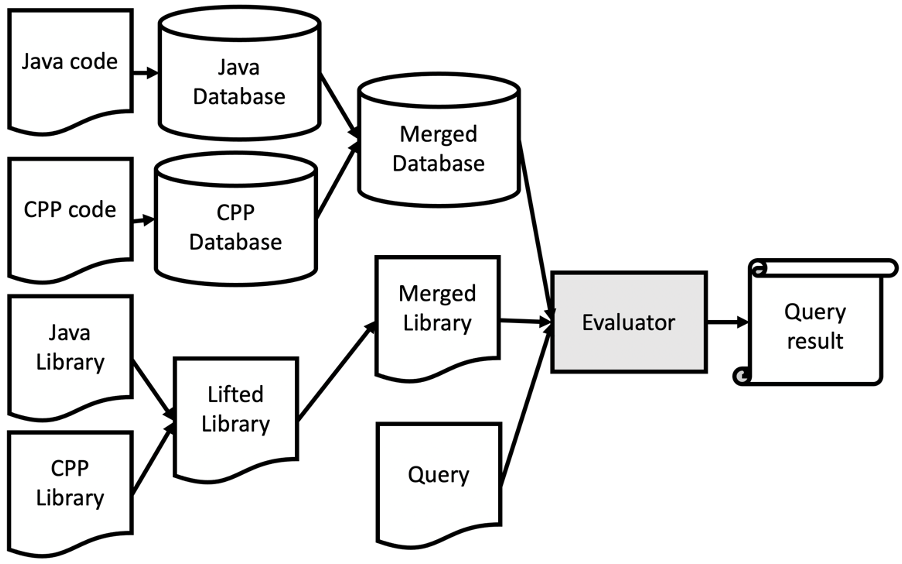
\includegraphics[width=0.5\textwidth]{img/Fig1}
Fig 1.

Figure 1. shows the overall structure of JN-QL. First, it generates database
for each language and merge it to one database. Then, two seperate dataflow
analysis library is also merged into one. Using the merged database and
merged library, the user can write a query and evaluate it to get query
result.

\subsection{Create database}
The first step is to gernerate database for each of two languages.  For
compiled languages such as C++ and Java, CodeQL generates database by tracing
the compiler for each language. While compiler is running, CodeQL extracts
information it needs, and create database with that information.  Creation of
database is performed in two steps: first, the extracted information from
compiler is stored in the human readable file format called trap files, and
second, these trap files are then converted into database.

[Insert example of trap file here]

JN-QL performs first step for each languages separately to get two sets of trap
files.  Next step would be to perfrom finalization step on merged set of trap
files. However, both of trap files have duplicated table, so simply mering them
would not work. The solution is to add prefix to name of each table. For
example, if both database have tables named "@expr", the table from cpp would
be renamed as "@cpp\_expr", and the table from java would be renamed as
"@java\_expr". After renaming each table, the second step can be applied to
finalize the database on which the query can be performed.

\subsection{Lift library}
CodeQL provides dataflow analysis library for each language: C++ and java.
Two dataflow analysis library have same structure, they share some classes such
as "Node", and some predicates such as "simpleLocalFlowStep".

Example:

class Node extends TNode {

  ...

}

predicate simpleLocalFlowStep(Node nodeFrom, Node nodeTo) {

  // Expr -> Expr
 
  exprToExprStep\_nocfg(
  
    nodeFrom.asExpr(),
    
    nodeTo.asExpr()
  
  )
  
  or
  
  // Assignment -> LValue post-update node
  
  ...

}

cpp/dataflow/internal/DataFlowUtil.qll

class Node extends TNode \{
   …
\}

predicate simpleLocalFlowStep(Node node1, Node node2) \{

  // Variable flow steps through
  
  // adjacent def-use and use-use pairs.
  
  exists(SsaExplicitUpdate upd |
  
    upd.getDefiningExpr().(VariableAssign).getSource()
    
    = node1.asExpr() or
    
    upd.getDefiningExpr().(AssignOp) = node1.asExpr()
  
  |
  
    node2.asExpr() = upd.getAFirstUse()
  
  )
  
  or
  
  // Flow through this
  
  ...

\}

cpp/dataflow/internal/DataFlowUtil.qll

However, since these two implementations are not compatible, that is,
we can not use "Node" class of C++ as an argument for "simpleLocalFlowStep" predicate of Java.
Therefore, we lift each of the library into the same level so that classes and predicates become compatible.
First, we encapsulated each of original dataflow into CodeQL's module, named CPP and JAVA so that
original classes and predicated can be separated with lifted ones.
A class can be lifted by first defining sum type, which denotes that the lifted class would be either from C++ or
Java, and then make the lifted class be of that type. We also implemented two member predicates that can cast
the lifted class into each of corresponding class.

private newtype TNode =

  TJavaNode(JAVA::Node n)
  
  or
  
  TCppNode(CPP::Node n)

class Node extends TNode \{
  
  JAVA::Node asJavaNode() \{
    
    this = TJavaNode(result)
  
  \}
  
  CPP::Node asCppNode() \{
    
    this = TCppNode(result)
  
  \}
  
  ...

\}

A predicate can be lifted by combining two original predicates with "or" connectives.
For each original predicate, each of the arguments and return values are casted down to
correspnding language's class. After lifting, the lifted predicate shows equlivalent behavior
as the original ones if all the arguments are from the same language.

predicate simpleLocalFlowStep(Node node1, Node node2) \{
  
  JAVA::simpleLocalFlowStep(
    
    node1.asJavaNode(), node2.asJavaNode()

  )
  
  or
  
  CPP::simpleLocalFlowStep(

    node1.asCppNode(), node2.asCppNode()

  )

\}

\subsection{Merge library}

After the library is lifted, the last step is to extend some predicates to reflect the
semantics of interoperation between languages. For example, the predicate named "viableCallable"
is a predicate for connecting function call and target function. It gets argument of class "DataFlowCall",
and the result is of class "DataFlowCallable". After merging the libraries, this predicate would be as follow:

DataFlowCallable viableCallable(DataFlowCall c) \{

result.asJavaDataFlowCallable()

  = JAVA::viableCallable(c.asJavaDataFlowCall()) or

result.asCppDataFlowCallable()

  = CPP::viableCallable(c.asCppDataFlowCall()) or

result.asCppDataFlowCallable()

  = viableCallableJ2C(c.asJavaDataFlowCall()) or

result.asJavaDataFlowCallable()

  = viableCallableC2J(c.asCppDataFlowCall())

\}

The first two lines are result of lifting, and they take advantage of the original predicates from dataflow library.
They handle the call edges from Java to Java, and from C++ to C++.
Next two lines are the result of merging library, and they are responsible for inter-language call edges.
The predicate "viableCallableJ2C" finds call edges from Java to C++. Since the function call targets for
these function calls can be statically determined, we don't need to use inner-flow analysis to implement this predicate.
Meanwhile, the predicate "viableCallableC2J" finds call edges from C++ to Java, and since runtime values are required to
determine the function call target, inner-flow is used to implment this predicate.
